
   %%%%%%%%%%%%%%%%%%%%%%%
 %%%  NOAH'S SUPER COOL  %%%
%%%%      ACADEMIC       %%%%
 %%%   LATEX TEMPLATE    %%%
   %%%%%%%%%%%%%%%%%%%%%%%

\documentclass[12pt]{article}
\usepackage[letterpaper]{geometry}
\geometry{top=1in, bottom=1in, left=1in, right=1in}
\usepackage{amsmath}
\usepackage{fontspec}
\usepackage{tgtermes}
\usepackage{hanging}
\usepackage{gensymb}
\setmainfont[
 ItalicFont={texgyretermes-italic.otf},
 BoldFont={texgyretermes-bold.otf},
 ]{texgyretermes-regular.otf}
\usepackage{setspace}
\doublespacing
\usepackage{graphicx}
\graphicspath{ {./graphics/} }

\begin{document}

% Title Page
\pagenumbering{gobble} % remove page numbers
\begin{center}
\topskip0pt
\vspace*{\fill}
Simple Harmonic Motion \\ Lab 12 - Noah Dinan \\ PHY 1110 - Mayer \\ \today \\
\vspace*{\fill}
\end{center}

\newpage
\pagenumbering{arabic} % resume page numbering
\setlength{\parindent}{0in}

\textbf{Results}\vspace{1em}

For this lab, we found the spring constant for springs attached to an air cart using both
Hooke's Law and the definition of a period $T$ for simple harmonic motion.

Hooke's Law simple states that $F=-kx$ which allowed us to graph $F$ and $x$ and measure the slope to find $k$.

For an object moving with a consistent period, we can determine period as shown below

\[ T = 2\pi [\sqrt{\frac{m}{k}}] \]

For the first part of the experiment, we measured the time taken for twenty periods and recorded the average
value for each period, this is shown in the table below. The largest potential for experimental error in this
experiment occurs during this step, we likely had some error in our timing.

\vspace{1em}
\begin{center}
    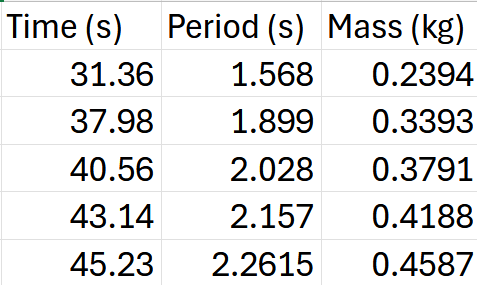
\includegraphics[scale=0.4]{table_12_1.png}
\end{center}
\vspace{1em}

By graphing $T^{2}$ on the y-axis and $m$ on the x-axis, the slope is $\frac{4\pi^{2}}{k}$ which we can 
rearrange to find $k$.

\vspace{1em}
\begin{center}
    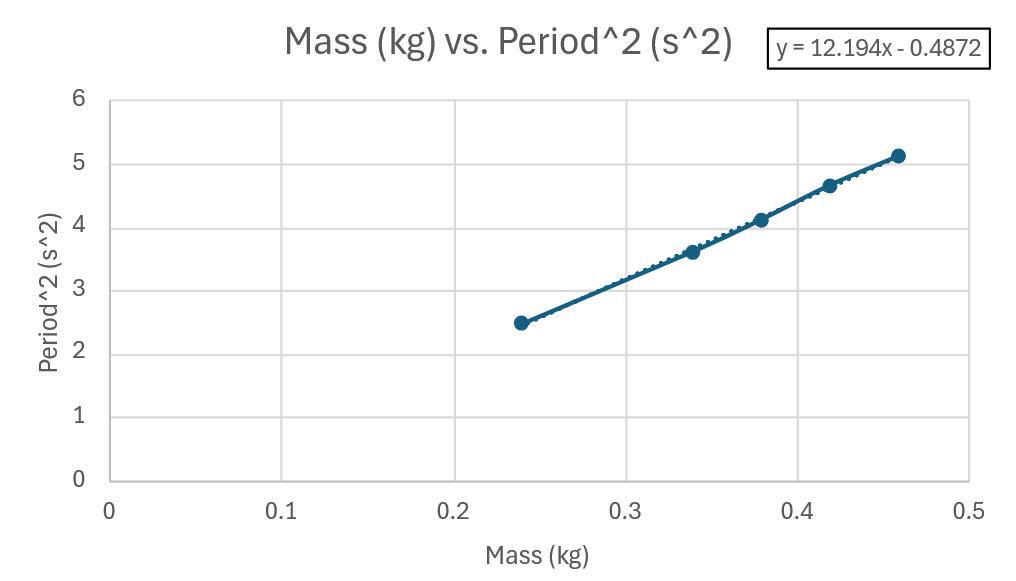
\includegraphics[scale=0.5]{graph_12_1.png}
\end{center}
\vspace{1em}

Based on this graph, with a slope of $12.194$, $k = \frac{4(\pi^2)}{12.194}$

\[ k_1 = 3.238 \text{Nm}^{-1} \]

Also based on this graph, we can find the x-intercept of the graph to be $\frac{-b}{m}$
where $m$ is the slope of the graph. This value should be negative one-third of the
mass of both springs which we found to be 0.0356 kilograms.

\[ \frac{-b}{m} = \frac{-0.4872}{12.194} = -0.0399 \]

This value is not $\frac{1}{3}$ of the mass but instead closer to the actual mass.
This discrepancy is likely due to an inaccurate measurement of the mass of the springs
or an inconsistent equilibrium point on the air track.

\newpage

For the second part of this experiment, we used the equation of Hooke's law to find a value for $k$.
For each row of the table below, we added 20 grams to a pulley and measured the displacement of the air cart
along the track. Another possible source of experimental error could have occurred while taking these measurements.

\vspace{1em}
\begin{center}
    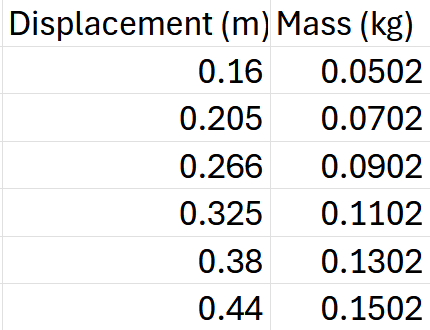
\includegraphics[scale=0.4]{table_12_2.png}
\end{center}
\vspace{1em}


Based on this data, we graphed $F$ on the y-axis, which was equal to $m * g$, and the displacement [$x$] on the x-axis.

\vspace{1em}
\begin{center}
    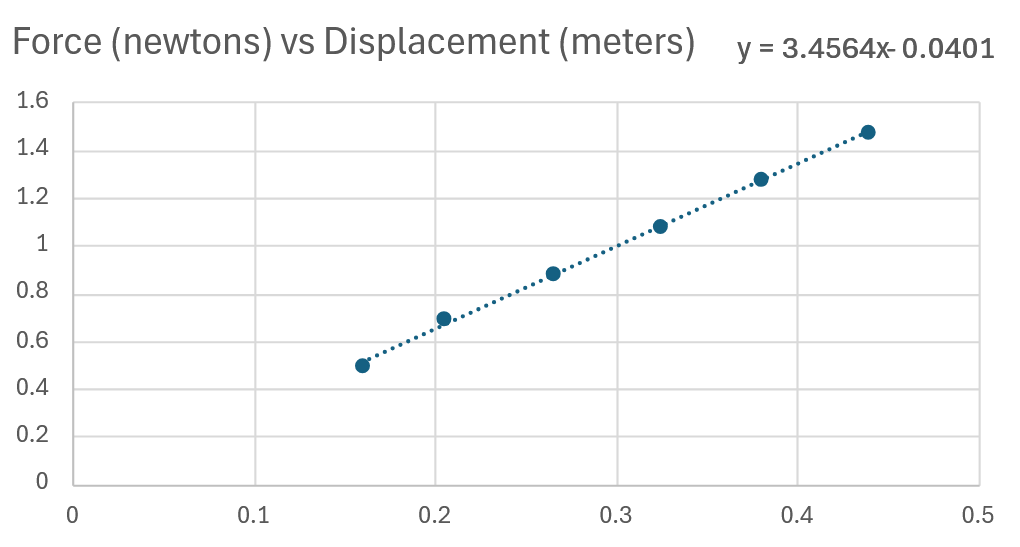
\includegraphics[scale=0.5]{graph_12_2.png}
\end{center}
\vspace{1em}

This gave us a slope of $k_2$.

\[ k_2 = 3.457 \text{Nm}^{-1} \]


\newpage

\textbf{Conclusions}\vspace{1em}

Our values for $k_1$ and $k_2$ were fairly close 3.238 vs 3.457 but may have been closer
if not for timing measurements errors that may have occurred in the first part of the
experiment.

\vspace{1em}

The inaccuracy seen in our x-intercept when compared to $\frac{1}{3}$ of the springs' masses
was likely because the offset of the graph as generated by Excel was incorrect or our mass measurements
for the springs were innacurate.

\end{document}
